\documentclass{beamer}
\usepackage{ctex}
\usepackage{amsmath}
\usepackage{amssymb}
\usepackage{amsthm}
\usetheme{metropolis}           % Use metropolis theme
\title{黄淮海地区小麦生长卫星遥感监测预测}
\date{\today}
\author{吴自华}
\institute{北京大学}
\begin{document}
  \maketitle
  \section{一、项目基本情况}
  \begin{frame}{基本信息}
    \begin{enumerate}
    	\item 隶属于国家重点研发计划项目“粮食丰产增效科技创新”
    	\item 起止时间:2016--2020
    \end{enumerate}
  \end{frame}
 
\begin{frame}{项目内容}
	\begin{enumerate}
		\item 黄淮海平原小麦空间分布监测
		\item 黄淮海平原小麦生长监测
		\item 黄淮海平原小麦产量预测
		\item 黄淮海平原土壤水分监测
		\item 黄淮海平原土壤养分监测
	\end{enumerate}
\end{frame}

\begin{frame}{任务要求}
	\begin{enumerate}
		\item 约束性指标:4套技术(文档、专题图、流程)
		\item 过程性指标:10类产品和数据
		\item 预期性指标:4类成果
	\end{enumerate}
\end{frame}

\section{二、项目完成情况}
\begin{frame}{已完成}
\begin{itemize}
	\item 县级、园区级专题图制作。任务书要求2017-2019年至少覆盖2个年度。在之前完成的2017-2018年专题图基础上,增补了2019年的作物长势专题图。
\end{itemize}
\end{frame}
\begin{frame}{进行中}
	\begin{enumerate}
		\item 2016、2019年省级专题图制作
		\item 省级土壤水分反演和精度验证
		\item 专利申请,等待受理通知书
		\item 现有的技术文档需要按照提交要求进行整理
	\end{enumerate}
\end{frame}
\begin{frame}{待完成}
	\begin{enumerate}
		\item 实验数据和文献资料整理
		\item 农气站土壤水分数据收集
		\item 软件著作权
	\end{enumerate}
\end{frame}
\section{三、项目年度进展}
\begin{frame}{总体}
\begin{enumerate}
	\item 按照项目任务书的要求,稳步推进需要每年进行的各项工作,如制作专题图、收集基础数据等。
	\item 利用Google Earth Engine实现了黄淮海平原小麦空间分布、长势监测等产品的自动化生产和处理,并提高了部分产品的空间分辨率。
\end{enumerate}
\end{frame}
\begin{frame}{野外实验}
\begin{columns}[c]
\column{6cm}
2019年3月14日至16日,项目组成员在河南省漯河市进行野外实验。测量的项目包括:
\begin{itemize}
	\item 叶面积指数
	\item SPAD
	\item 株高
	\item 株密度
\end{itemize}
采集的植株和土壤样本,经化验分析后得到:
\begin{itemize}
	\item 植株生物量
	\item 植株含氮量
	\item 土壤水分
\end{itemize}
\column{4cm}
\begin{figure}
	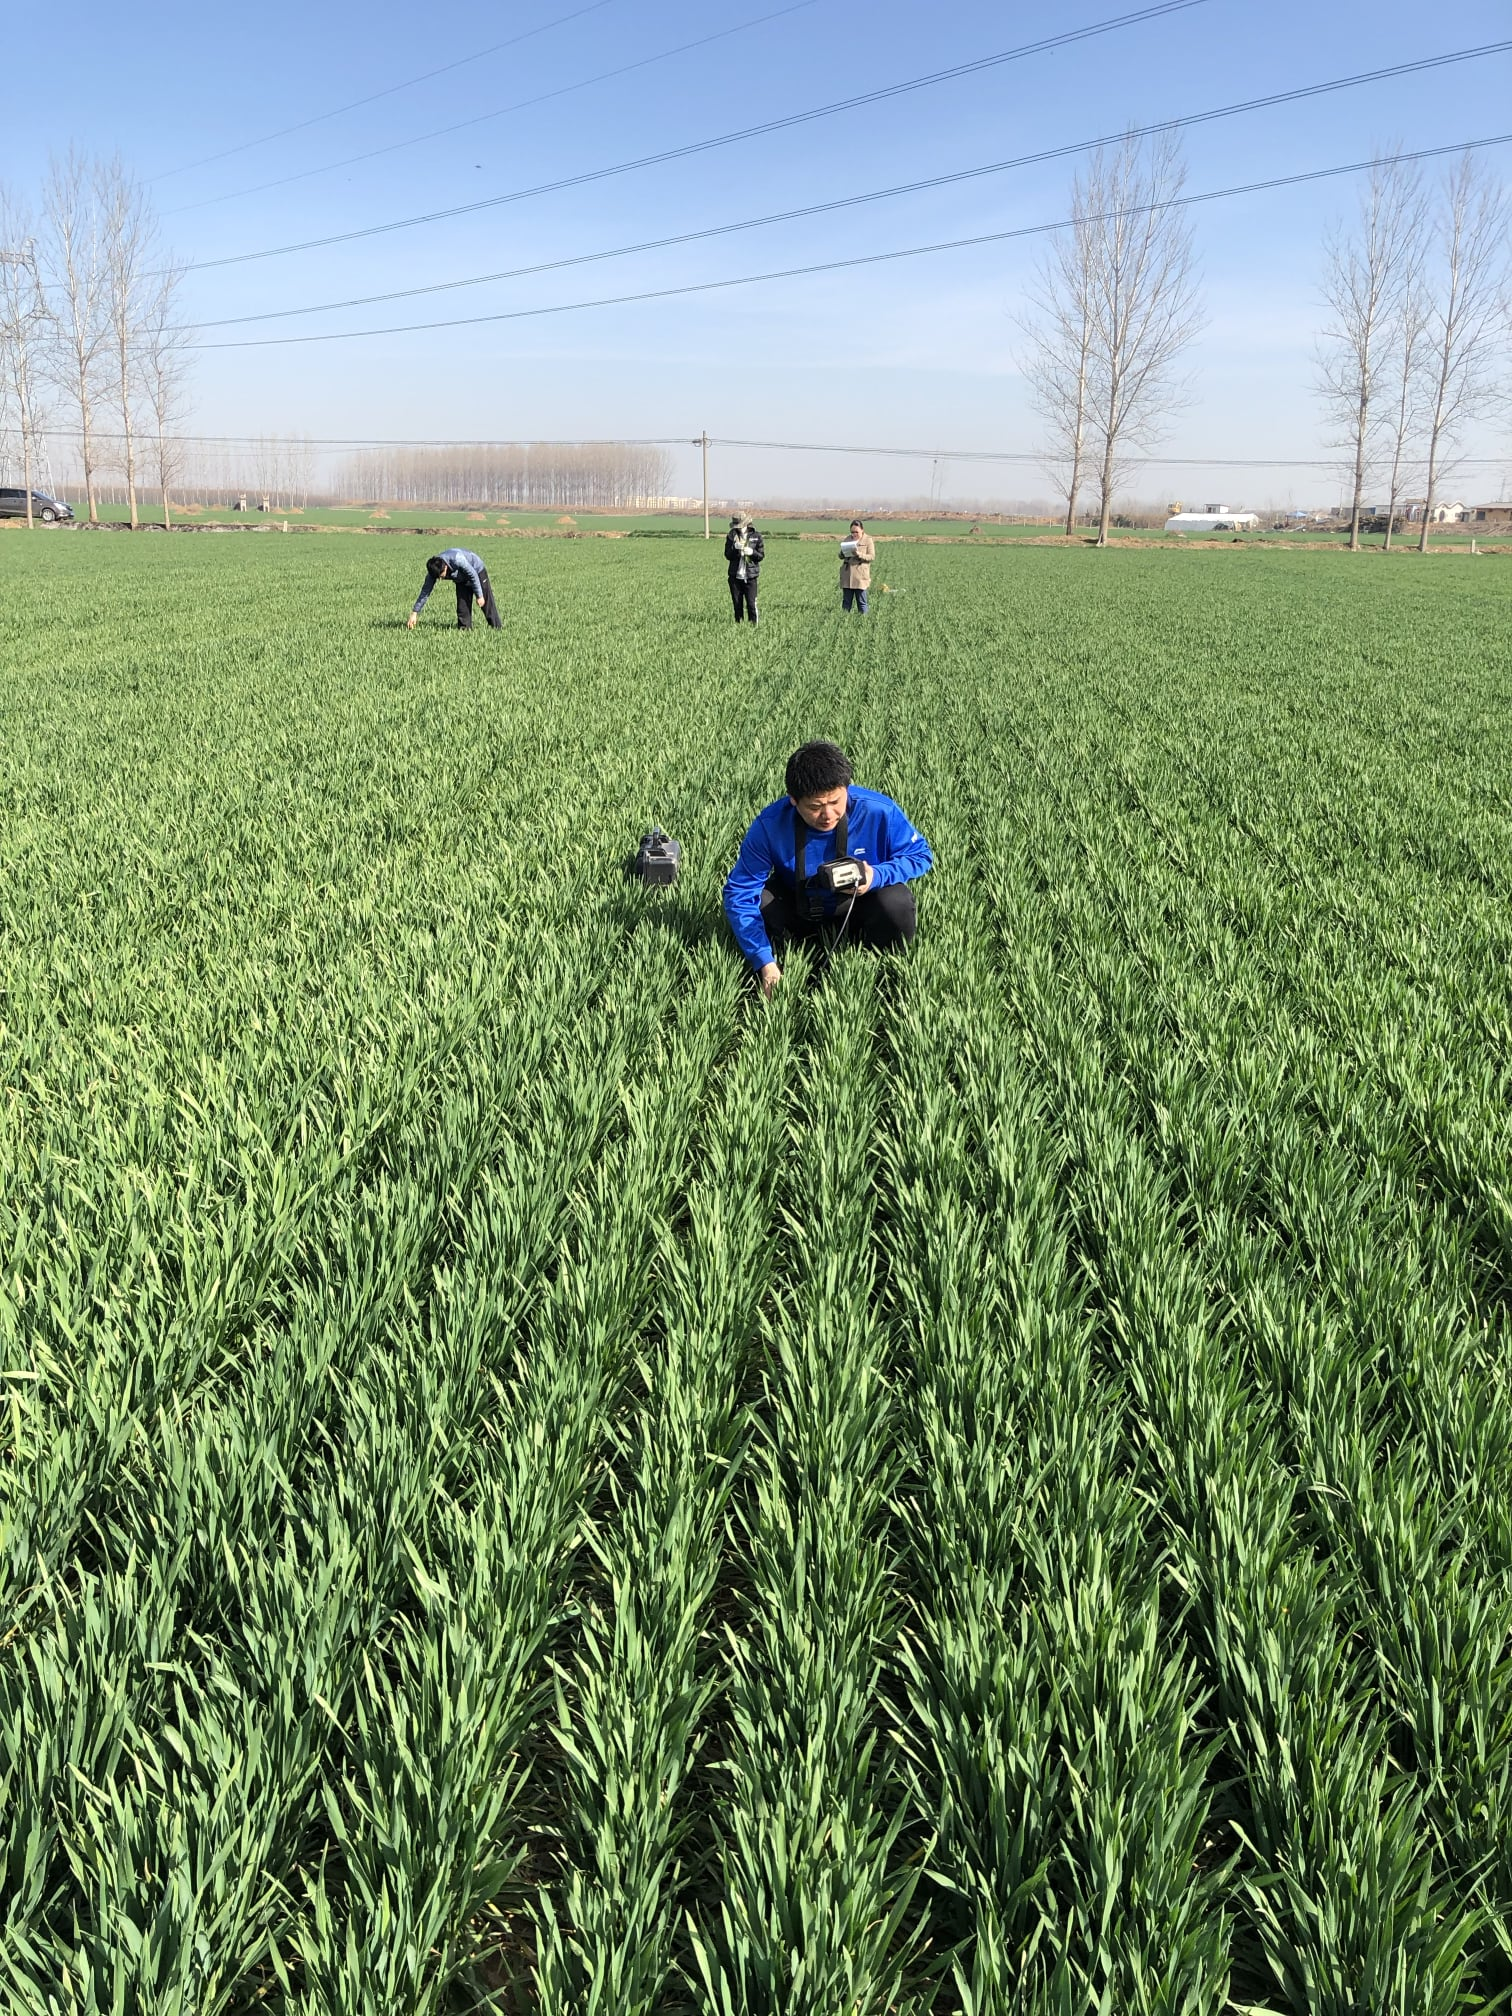
\includegraphics[height=6cm]{images/field.jpg}
\end{figure}
\end{columns}
\end{frame}
\begin{frame}{空间分布}
\begin{columns}
\column{4.5cm}
\begin{itemize}
	\item 原方法:基于两个时相的NDVI阈值。省级使用MODIS,县级和园区级使用Sentinel-2。
	\item 新方法:利用两个时相各6个波段+NDVI共14个输入参数,使用随机森林方法进行分类。整个计算和处理过程在GEE平台完成,提高了省级空间分布产品的空间分辨率。
	\item 验证:目视解译
\end{itemize}
\column{6cm}
\begin{figure}
	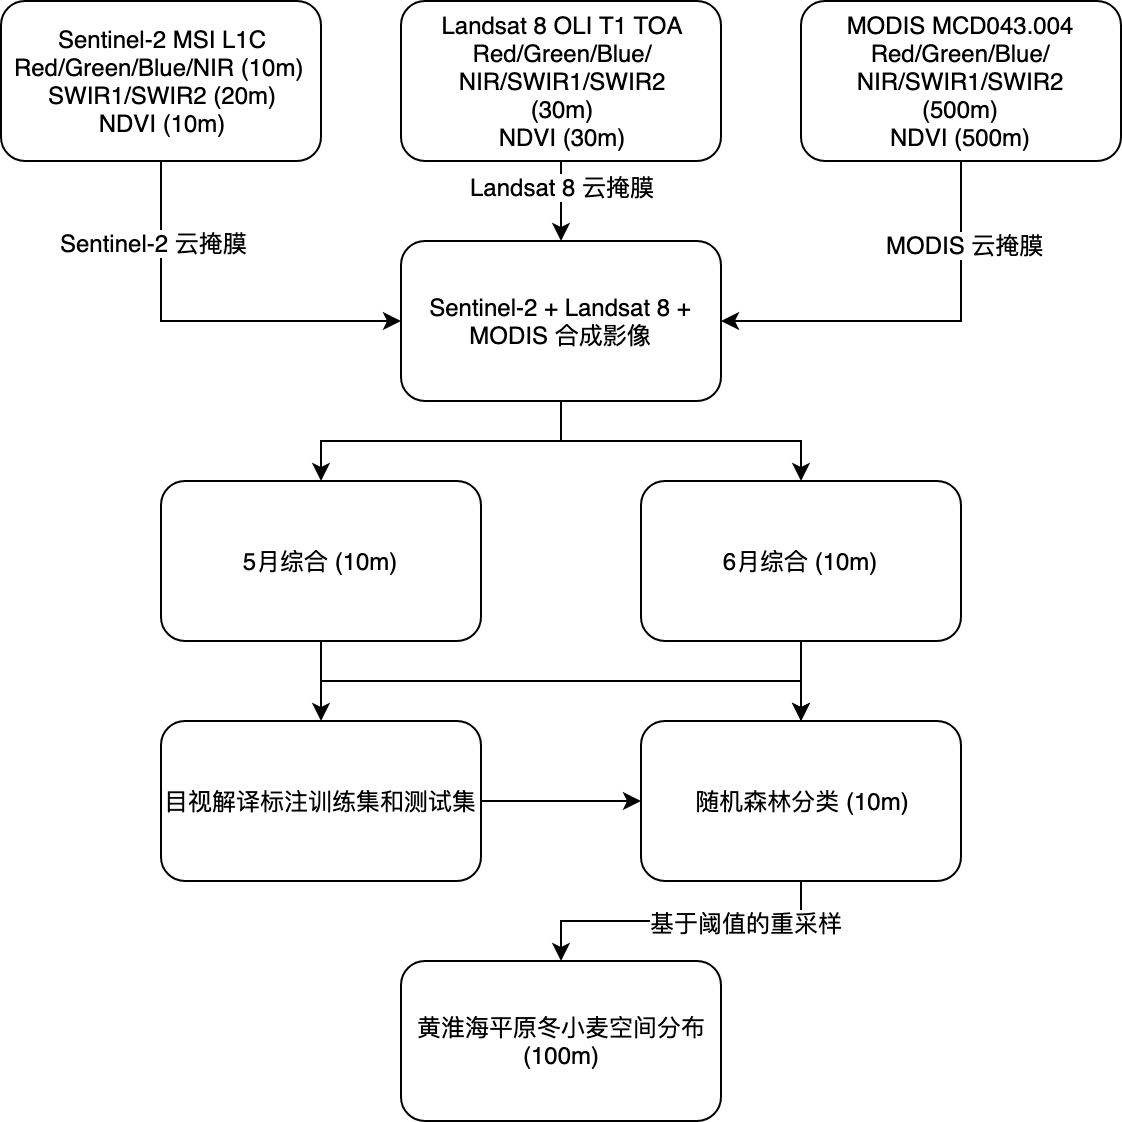
\includegraphics[height=6cm]{images/area.png}
\end{figure}
\end{columns}
\end{frame}
\begin{frame}{生长监测}
对小麦生长过程中的四个重要的长势参数进行监测,包括
\begin{enumerate}
	\item 叶面积指数
	\item 生物量
	\item 冠层氮含量
	\item 冠层氮累积量
\end{enumerate}
\end{frame}
\begin{frame}{生长监测--叶面积指数}
采用IDVI和NDVI加权的统计回归模型。使用实测数据进行验证。

\begin{block}{计算公式}
	\begin{equation}
	\mathrm{IDVI}=\frac{1-\rho_{\mathrm{red}}+\rho_{\mathrm{nir}}}{1-\rho_{\mathrm{red}}-\rho_{\mathrm{nir}}}
	\end{equation}
	\begin{equation}
	\alpha=\frac{1}{1+e^{-k(\mathrm{NDVI}-\mathrm{NDVI}_t}}
	\end{equation}
	\begin{equation}
	\mathrm{LAI_{estimation}}=(1-\alpha)\mathrm{LAI_{NDVI}}+\alpha\mathrm{LAI_{IDVI}}
	\end{equation}
\end{block}

\end{frame}
\begin{frame}{生长监测-氮含量}
	\begin{block}{省级}
		\begin{itemize}
			\item 数据:MODIS
			\item 方法:基于MRVI统计回归
			\item 验证:实测数据
		\end{itemize}
	\end{block}
	
	\begin{block}{县级、园区级}
		\begin{itemize}
			\item 数据:Sentinel-2
			\item 方法:人工神经网络
			\item 验证:实测数据
		\end{itemize}
	\end{block}
\end{frame}
\begin{frame}{生长监测-生物量}
	\begin{block}{省级}
	\begin{itemize}
		\item 数据:Himawari、MODIS
		\item 方法:光热水肥四要素计算GPP,利用经验系数转换得到生物量
	\end{itemize}
\end{block}

\begin{block}{县级、园区级}
	\begin{itemize}
		\item 数据:Sentinel-2
		\item 方法:NDRE统计回归
		\item 验证:实测数据
	\end{itemize}
\end{block}
\end{frame}
\begin{frame}{生长监测-氮累积量}
	\begin{block}{计算方法}
		\begin{equation}
			\mathrm{TNC} = \mathrm{CNC}\times\mathrm{AGB}
		\end{equation}
	\end{block}
\end{frame}
\begin{frame}{产量预测}
		\begin{block}{省级}
		\begin{itemize}
			\item 数据:Himawari、MODIS
			\item 方法:光热水肥四要素计算GPP,利用光能利用率等经验系数得到生物量,再利用收获系数等经验系数计算得到产量
			\item 光:Himawari PAR + MODIS FPAR
			\item 热:MODIS ScaledLST
			\item 水:MODIS ScaledVSDI
			\item 肥:MODIS MRVI
		\end{itemize}
	\end{block}
	
	\begin{block}{县级、园区级}
		\begin{itemize}
			\item 数据:Sentinel-2
			\item 方法:EVI时序最大值统计回归
			\item 验证:实测数据
		\end{itemize}
	\end{block}
\end{frame}
\begin{frame}{土壤水分}
		\begin{block}{省级}
		\begin{itemize}
			\item 数据:AMSR-2、SMAP、MODIS等
			\item 方法:\textbf{研究开展中}
		\end{itemize}
	\end{block}
	
	\begin{block}{县级、园区级}
		\begin{itemize}
			\item 数据:Sentinel-1
			\item 方法:$\alpha$-近似模型+SVR
			\item 验证:实测数据
		\end{itemize}
	\end{block}
\end{frame}
\begin{frame}{土壤养分}
	\begin{block}{县级、园区级}
		\begin{itemize}
			\item 数据:Sentinel-2
			\item 方法:REB1+NIR二元统计回归
			\item 验证:实测数据
		\end{itemize}
	\end{block}
\end{frame}
\section{四、存在问题}
\begin{frame}{目前存在的主要问题}
对照任务书要求,本项目主要还存在以下问题:
\begin{enumerate}
	\item 暂时还没有找到2016-2019年农业气象站土壤水分观测数据的获取途径。
	\item 省级土壤水分产品的生产。
	\item 省级产量、土壤水分产品的精度验证。
	\item 地面调查数据集、文献资料收集数据集的整理。
\end{enumerate}
\end{frame}
\section{五、下一步工作计划}
\begin{frame}{下一步工作计划}
	\begin{enumerate}
		\item 完成2019年年度进展报告初稿(本周)
		\item 完成2019年省级专题图制作(下周)
		\item 整理地面调查数据集、文献资料收集数据集(下周)
		\item 各部分技术文档整理和修改(下两周)
		\item 软件著作权申请
	\end{enumerate}
\end{frame}
\end{document}